\documentclass[11pt]{article}
\usepackage[margin=0.8in]{geometry}
\usepackage{amsmath,amssymb,graphicx,booktabs,natbib,hyperref,placeins}
\newcommand{\btheta}{\boldsymbol{\theta}}
\graphicspath{{../figures/}}
\title{Identifiability and finite-sample bias in group-testing calibration}
\author{Reproducibility analysis for the JRSSA revision}
\date{10 November 2026}
\begin{document}\maketitle
\noindent This note distinguishes structural identifiability from information adequacy and finite-sample estimation. All calculations use R and the same three-parameter pooled-test model. Complete code and results are available at \url{https://github.com/chikuang/JRSSA-group-testing-reproducibility}.
\section{Statistical arguments}
\subsection{When a pooled-only design cannot identify the parameters}\label{app:identifiability}
Write $p=p_0$, $s=p_1$, $t=p_2$, and $a=s+t-1$. The model is
\[
 \pi_x=s-a(1-p)^x,\qquad
 Y_x\mathrel{\mathop\sim^{\rm ind}}\operatorname{Binomial}(n_x,\pi_x).
\]
The following statements concern joint estimation of $(p,s,t)$ from regular pooled assays only, with pool-size-invariant accuracy and no external calibration information. We assume $0<p<1$ and $1/2<s,t<1$. The requirement for at least three distinct group sizes is established in \citet{huang:2017:design-group}; the argument below makes its consequences for bias explicit.

Let $K$ be the number of distinct pool sizes with positive counts. With $f_x=\partial\pi_x/\partial(p,s,t)$,
\[
 J=\sum_x \frac{n_x f_x f_x^{\mathsf T}}{\pi_x(1-\pi_x)},\qquad
 \operatorname{rank}(J)\leq K.
\]
Thus $K=1$ or $2$ cannot give nonsingular information for all three parameters. More directly, with one pool size $m$, the data determine only the combination $s-a(1-p)^m$. With two sizes $x_1<x_2$, suppose their population probabilities are $v_1<v_2$. For any nearby prevalence $p$, define
\begin{equation}\label{eq:identification-ridge}
 z_i=(1-p)^{x_i},\quad
 a(p)=\frac{v_2-v_1}{z_1-z_2},\quad
 s(p)=v_1+a(p)z_1,\quad t(p)=1+a(p)-s(p).
\end{equation}
Continuity ensures that an interval of such parameter vectors remains inside the parameter space whenever the original vector is interior. Each vector gives exactly the same pair $(v_1,v_2)$ and hence the same distribution of all observations, for every choice of positive counts $n_{x_1}$ and $n_{x_2}$. Increasing these counts cannot identify the missing direction.

For example, at sizes $1$ and $15$, the two vectors
\[
 \begin{aligned}
 (p,s,t)&=(0.022,0.92,0.965),\\
 (p',s',t')&=(0.025,0.8305789474,0.9654302294)
 \end{aligned}
\]
give the same positive-test probabilities (to the displayed precision). Prevalence and sensitivity cannot be separated by these observations alone.

\paragraph{Implication for bias and consistency.}
Let $\theta\ne\theta'$ give the same data distribution under the design. For any estimator $T_j$ with finite expectation, $E_\theta T_j=E_{\theta'}T_j=\mu_j$, and therefore
\begin{equation}\label{eq:nonident-bias-bound}
 \max\{|\mu_j-\theta_j|,|\mu_j-\theta'_j|\}
 \geq\tfrac12|\theta_j-\theta'_j|.
\end{equation}
Whenever the two component values differ, no estimator can be unbiased at both parameter points. The same indistinguishability also rules out consistency at both points as the budget increases. This is a consequence of nonidentifiability, rather than a general property of non-optimal allocations. A numerical optimiser can return a point on the likelihood ridge, but its selection rule supplies information that the data do not contain.

\paragraph{Three distinct sizes and weak information.}
For three sizes $x_1<x_2<x_3$, put $\lambda=-\log(1-p)>0$, $A=x_2-x_1$ and $B=x_3-x_1$. Then
\[
 \frac{\pi_{x_2}-\pi_{x_1}}{\pi_{x_3}-\pi_{x_1}}
 =\frac{1-e^{-A\lambda}}{1-e^{-B\lambda}},\qquad 0<A<B.
\]
The logarithmic derivative of the right-hand side is
$A/(e^{A\lambda}-1)-B/(e^{B\lambda}-1)>0$, since $u/(e^{u\lambda}-1)$ decreases strictly in $u>0$. Consequently the three population probabilities identify $p$ uniquely, after which \eqref{eq:identification-ridge} identifies $s$ and $t$. The same calculation gives a nonsingular local Jacobian. Positive allocation to any three distinct sizes therefore identifies the interior model; additional sizes may improve information or support model checking.

Identification does not ensure adequate precision at a given budget. At low prevalence or over a narrow range of pool sizes, the information can be poorly conditioned despite having rank three. Accuracy constraints may then be active in many repeated samples. At the excluded limiting configurations $p=0$, $p=1$ or $s+t=1$, some parameter directions again disappear. Similarly, rounding a support count to zero can turn a nominally identifiable design into one with fewer than three observed sizes. Known accuracy parameters or appropriately designed validation data change the identification problem and can remove the need for three regular-assay pool sizes.

\begin{table}[!htbp]
\centering\small
\caption{Identifiability and information at the same budget of 500 assays, with $(p_0,p_1,p_2)=(0.022,0.92,0.965)$. Information rank is evaluated under the three-parameter, pool-size-invariant model. Relative $D$-efficiency uses the displayed $(1,7,15)$ allocation as its reference. A rank-three design is identifiable but need not be informative at the available budget.}\label{tab:identification-comparison}
\begin{tabular}{llcr}\toprule
Pool sizes & Counts & Information rank & Relative $D$-efficiency\\\midrule
10 & 500 & 1 & 0\\
1, 15 & 250, 250 & 2 & 0\\
1, 2, 3 & 167, 167, 166 & 3 & 0.0415\\
1, 7, 15 & 167, 167, 166 & 3 & 1.0000\\
1, 6, 10, 15 & 125, 125, 125, 125 & 3 & 0.9092\\
\bottomrule\end{tabular}
\end{table}
\subsection{Finite-sample bias under identifiable designs}\label{app:finite-bias-theory}
For a fixed identifiable design under the correctly specified model, the expected likelihood score is zero. This property does not imply that the root of the score equation is an unbiased estimator. Under regular interior asymptotics with positive limiting allocations, the joint MLE is consistent and its leading bias is generally of order $C^{-1}$; its coefficient depends on the design and the parameter vector. Information criteria such as $D$-optimality concern the leading covariance, rather than this bias coefficient. Boundary and weak-information settings need a separate finite-sample assessment.

A simple submodel shows explicitly how a pooled-data MLE can be biased. Suppose sensitivity and specificity are both known to equal one, all pools have size $m>1$, and $Y\sim\operatorname{Binomial}(n,\pi)$ with $\pi=1-(1-p)^m$. The MLE is $\hat p=g(Y/n)$, where $g(u)=1-(1-u)^{1/m}$ is strictly convex. Jensen's inequality gives $E(\hat p)>p$ for $0<p<1$ and finite $n$. For fixed interior $p$,
\begin{equation}\label{eq:jensen-pooling-bias}
 E(\hat p)-p
 =\frac{m-1}{2m^2 n}\,\pi(1-\pi)^{1/m-1}+o(n^{-1}).
\end{equation}
For $m=10$ and $p=0.022$, exact binomial summation gives biases $1.106\times10^{-4}$, $2.197\times10^{-5}$ and $5.485\times10^{-6}$ at $n=100$, $500$ and $2000$. This illustration establishes a source of finite-sample bias even when the relevant parameter is identified. It neither establishes that every non-optimal design has larger bias nor provides the bias formula for the joint three-parameter MLE. Bias correction with known imperfect assay accuracy is studied by \citet{hepworth:2021:bias}; that assumption differs from joint calibration here.

\section{Matched-budget Monte Carlo study}
\subsection{Simulation specification and numerical assessment}\label{app:bias-simulation}
We compared rounded locally $D$-optimal allocations with an identifiable four-size uniform comparator under the same resource constraint and the same joint estimator. In the cost setting, $(p,s,t)=(0.07,0.93,0.96)$, the admissible sizes are $1,\ldots,61$, $c(x)=0.8+0.2x$ and $C\in\{100,500,2000\}$. In the low-prevalence setting, $(p,s,t)=(0.022,0.92,0.965)$, the admissible sizes are $1,\ldots,15$, $c(x)=1$ and the assay budgets are $500$, $2000$ and $10000$. These settings and budgets were fixed before examining the simulation outcomes. The local design parameters equal the generating parameters; this comparison does not assess misspecified nominal values.

The approximate $D$-optimal supports are $(1,10,61)$ and $(1,7,15)$. CVXR with CLARABEL was applied after a nonsingular coordinate transformation; full-candidate relative directional residuals are below $1.2\times10^{-5}$. For the simulation, integer counts were chosen by enumerating fully spent allocations on these supports with the second and third counts within six of their unrounded values, selecting the largest determinant. This rounding procedure differs from the local-search comparison in the separate revision rounding analysis; it does not certify global integer optimality. The comparator uses $(1,21,41,61)$ or $(1,6,10,15)$ and counts closest to equal subject to spending exactly the same budget. All allocations have positive-definite information. Table~\ref{tab:bias-allocations} reports their assay and specimen totals: matching the binding resource does not require both totals to agree.

For each of the twelve cells we generated $R=10000$ independent datasets. We maximised the same binomial log likelihood over $p\in[10^{-7},1-10^{-7}]$ and $s,t\in[0.5,1]$, approximating the closure of the manuscript parameter space. Optimisation used log prevalence, analytic gradients, and starting prevalences $0.003$, $0.02$, $0.10$ and $0.40$ with data-derived accuracy starts. A feasible saturated solution for three observed sizes attains the global binomial maximum and was used directly. Other samples used constrained optimisation and numerical polishing. The generating parameters were not supplied to the fitting routine. All boundary estimates were retained.

We report empirical bias $R^{-1}\sum_r(\hat\theta_{rj}-\theta_j)$, sample variance with denominator $R-1$, and RMSE $\{R^{-1}\sum_r(\hat\theta_{rj}-\theta_j)^2\}^{1/2}$. Thus the exact empirical decomposition uses $(R-1)/R$ times the sample variance. The bias Monte Carlo SE is the empirical standard deviation divided by $\sqrt R$. Variance Monte Carlo SE uses the empirical standard deviation of squared centred estimates divided by $\sqrt R$; RMSE Monte Carlo SE uses the delta method applied to mean squared error. Tables~\ref{tab:bias-cost-full} and~\ref{tab:bias-low-full} give all results; Figures~\ref{fig:bias-cost} and~\ref{fig:bias-low} display the corresponding budget trends.

There were 832 nonzero optimiser termination codes among 120000 retained estimates. Expanded starting grids checked these cases, every projected-gradient flag and the first 50 datasets per cell; no log-likelihood improvement exceeded $2\times10^{-9}$. An independent audit profiled prevalence over a grid, solving the concave accuracy subproblem at each prevalence and refining profile minima. It checked the first 50 datasets per cell and every projected-gradient value above $10^{-3}$, with maximum improvement below $1.8\times10^{-9}$. Across all fits, the maximum projected gradient divided by assay count was below $5.3\times10^{-6}$. No replicate was discarded. Table~\ref{tab:bias-diagnostics} reports termination flags and boundary frequencies. The random seed was 20261110, using independent L'Ecuyer--CMRG streams; code, generated counts, estimates and session information are provided in the paper's reproducibility repository.

At $C=500$ in the cost setting, $D$ reduces prevalence and specificity RMSE, whereas the uniform comparator has lower sensitivity RMSE. At 500 assays in the low-prevalence setting, sensitivity bias is approximately $-0.143$ under both designs and an accuracy boundary is reached in about 88\% of samples. Boundary frequencies remain about 53\% at 10000 assays. These findings distinguish improved allocation from sufficient information: local $D$-optimality does not guarantee small finite-sample bias or coordinatewise RMSE dominance. They also show why a finite-sample variance below an inverse-information bound for regular unbiased estimation need not contradict that bound: the bounded estimators here can be strongly biased and frequently reach the boundary.

\begin{table}[!htbp]\centering\scriptsize
\caption{Cost budgets, $(p,s,t)=(0.07,0.93,0.96)$ and $q=0.2$. Bias and RMSE are in percentage points, variance in squared percentage points; parentheses give Monte Carlo SEs. Each row uses 10000 replicates.}\label{tab:bias-cost-full}
\begin{tabular}{rllrrr}\toprule
Budget & Parameter & Design & Bias (MCSE) & Variance (MCSE) & RMSE (MCSE)\\\midrule
100 & Prevalence & D & 0.684 (0.041) & 17.111 (0.497) & 4.192 (0.064) \\
100 & Sensitivity & D & 0.859 (0.126) & 157.596 (2.890) & 12.582 (0.107) \\
100 & Specificity & D & -0.251 (0.050) & 24.953 (0.433) & 5.001 (0.045) \\
100 & Prevalence & U4 & 3.263 (0.089) & 79.347 (2.542) & 9.486 (0.159) \\
100 & Sensitivity & U4 & 2.143 (0.086) & 73.122 (1.630) & 8.815 (0.076) \\
100 & Specificity & U4 & -1.334 (0.099) & 98.118 (2.457) & 9.994 (0.134) \\
500 & Prevalence & D & 0.307 (0.019) & 3.631 (0.075) & 1.930 (0.021) \\
500 & Sensitivity & D & -0.193 (0.074) & 54.440 (0.887) & 7.381 (0.061) \\
500 & Specificity & D & 0.140 (0.029) & 8.343 (0.112) & 2.892 (0.019) \\
500 & Prevalence & U4 & 0.838 (0.037) & 13.855 (0.481) & 3.815 (0.069) \\
500 & Sensitivity & U4 & 1.124 (0.055) & 30.367 (0.404) & 5.624 (0.031) \\
500 & Specificity & U4 & -0.589 (0.061) & 37.714 (0.771) & 6.169 (0.067) \\
2000 & Prevalence & D & 0.065 (0.010) & 0.965 (0.015) & 0.984 (0.008) \\
2000 & Sensitivity & D & 0.127 (0.042) & 17.620 (0.247) & 4.199 (0.029) \\
2000 & Specificity & D & 0.043 (0.016) & 2.572 (0.035) & 1.604 (0.011) \\
2000 & Prevalence & U4 & 0.196 (0.017) & 2.943 (0.074) & 1.727 (0.023) \\
2000 & Sensitivity & U4 & 0.534 (0.035) & 12.117 (0.152) & 3.521 (0.022) \\
2000 & Specificity & U4 & -0.091 (0.037) & 13.531 (0.204) & 3.679 (0.028) \\

\bottomrule\end{tabular}\end{table}
\begin{table}[!htbp]\centering\scriptsize
\caption{Assay budgets, $(p,s,t)=(0.022,0.92,0.965)$. Bias and RMSE are in percentage points, variance in squared percentage points; parentheses give Monte Carlo SEs. Each row uses 10000 replicates.}\label{tab:bias-low-full}
\begin{tabular}{rllrrr}\toprule
Budget & Parameter & Design & Bias (MCSE) & Variance (MCSE) & RMSE (MCSE)\\\midrule
500 & Prevalence & D & 1.064 (0.015) & 2.306 (0.024) & 1.854 (0.014) \\
500 & Sensitivity & D & -14.345 (0.237) & 561.812 (1.896) & 27.705 (0.145) \\
500 & Specificity & D & 0.239 (0.019) & 3.674 (0.051) & 1.931 (0.013) \\
500 & Prevalence & U4 & 1.018 (0.015) & 2.189 (0.023) & 1.796 (0.013) \\
500 & Sensitivity & U4 & -14.265 (0.238) & 564.740 (1.887) & 27.716 (0.146) \\
500 & Specificity & U4 & 0.195 (0.021) & 4.605 (0.064) & 2.155 (0.014) \\
2000 & Prevalence & D & 0.893 (0.013) & 1.733 (0.015) & 1.591 (0.011) \\
2000 & Sensitivity & D & -12.546 (0.224) & 502.265 (2.553) & 25.683 (0.146) \\
2000 & Specificity & D & 0.190 (0.010) & 1.001 (0.014) & 1.018 (0.007) \\
2000 & Prevalence & U4 & 0.923 (0.013) & 1.739 (0.014) & 1.610 (0.011) \\
2000 & Sensitivity & U4 & -13.287 (0.226) & 511.744 (2.361) & 26.234 (0.145) \\
2000 & Specificity & U4 & 0.192 (0.011) & 1.310 (0.019) & 1.160 (0.008) \\
10000 & Prevalence & D & 0.577 (0.010) & 1.007 (0.013) & 1.158 (0.010) \\
10000 & Sensitivity & D & -9.067 (0.190) & 360.909 (2.929) & 21.050 (0.138) \\
10000 & Specificity & D & 0.115 (0.005) & 0.216 (0.003) & 0.478 (0.003) \\
10000 & Prevalence & U4 & 0.625 (0.010) & 1.064 (0.013) & 1.206 (0.010) \\
10000 & Sensitivity & U4 & -9.935 (0.195) & 380.231 (2.875) & 21.884 (0.139) \\
10000 & Specificity & U4 & 0.129 (0.005) & 0.281 (0.004) & 0.545 (0.004) \\

\bottomrule\end{tabular}\end{table}
\begin{table}[!htbp]\centering\scriptsize
\caption{Implemented allocations and approximate-design $D$-efficiency. A pair $x:n$ denotes $n$ assays at pool size $x$. Expenditure equals the stated budget in every row.}\label{tab:bias-allocations}
\begin{tabular}{lrl lrrr}\toprule
Setting & Budget & Design & Pool size:count & Assays & Specimens & $D$-eff.\\\midrule
Cost &   100 & D & 1:33; 10:10; 61:3 &    46 &   316 & 0.9909 \\
Cost &   100 & U4 & 1:5; 21:4; 41:4; 61:3 &    16 &   436 & 0.4870 \\
Cost &   500 & D & 1:163; 10:60; 61:13 &   236 &  1556 & 0.9999 \\
Cost &   500 & U4 & 1:19; 21:17; 41:18; 61:18 &    72 &  2212 & 0.4385 \\
Cost &  2000 & D & 1:665; 10:240; 61:51 &   956 &  6176 & 1.0000 \\
Cost &  2000 & U4 & 1:70; 21:71; 41:71; 61:72 &   284 &  8864 & 0.4311 \\
Low &   500 & D & 1:166; 7:167; 15:167 &   500 &  3840 & 1.0000 \\
Low &   500 & U4 & 1:125; 6:125; 10:125; 15:125 &   500 &  4000 & 0.9092 \\
Low &  2000 & D & 1:667; 7:667; 15:666 &  2000 & 15326 & 1.0000 \\
Low &  2000 & U4 & 1:500; 6:500; 10:500; 15:500 &  2000 & 16000 & 0.9092 \\
Low & 10000 & D & 1:3333; 7:3333; 15:3334 & 10000 & 76674 & 1.0000 \\
Low & 10000 & U4 & 1:2500; 6:2500; 10:2500; 15:2500 & 10000 & 80000 & 0.9092 \\

\bottomrule\end{tabular}\end{table}
\begin{table}[!htbp]\centering\small
\caption{Numerical and boundary diagnostics, each based on 10000 fits. Flags are nonzero numerical optimiser termination codes, not omitted estimates. The final column gives the maximum projected gradient divided by assay count.}\label{tab:bias-diagnostics}
\begin{tabular}{lrlrrr}\toprule
Setting & Budget & Design & Flags & Accuracy boundary (\%) & Max.~gradient\\\midrule
Cost &   100 & D &  67 & 89.98 & 1.3e-07 \\
Cost &   100 & U4 & 360 & 94.88 & 5.3e-06 \\
Cost &  2000 & D &   2 & 5.25 & 5.5e-08 \\
Cost &  2000 & U4 &  41 & 24.89 & 2.9e-07 \\
Cost &   500 & D &  48 & 43.44 & 1.0e-07 \\
Cost &   500 & U4 &  55 & 62.77 & 1.7e-07 \\
Low & 10000 & D &  45 & 53.00 & 1.4e-07 \\
Low & 10000 & U4 &  46 & 53.76 & 7.3e-07 \\
Low &  2000 & D &  25 & 73.62 & 5.0e-08 \\
Low &  2000 & U4 &  53 & 74.98 & 3.0e-07 \\
Low &   500 & D &  45 & 87.55 & 1.8e-07 \\
Low &   500 & U4 &  45 & 88.30 & 3.2e-07 \\
\bottomrule\end{tabular}\end{table}
\begin{figure}[!htbp]\centering
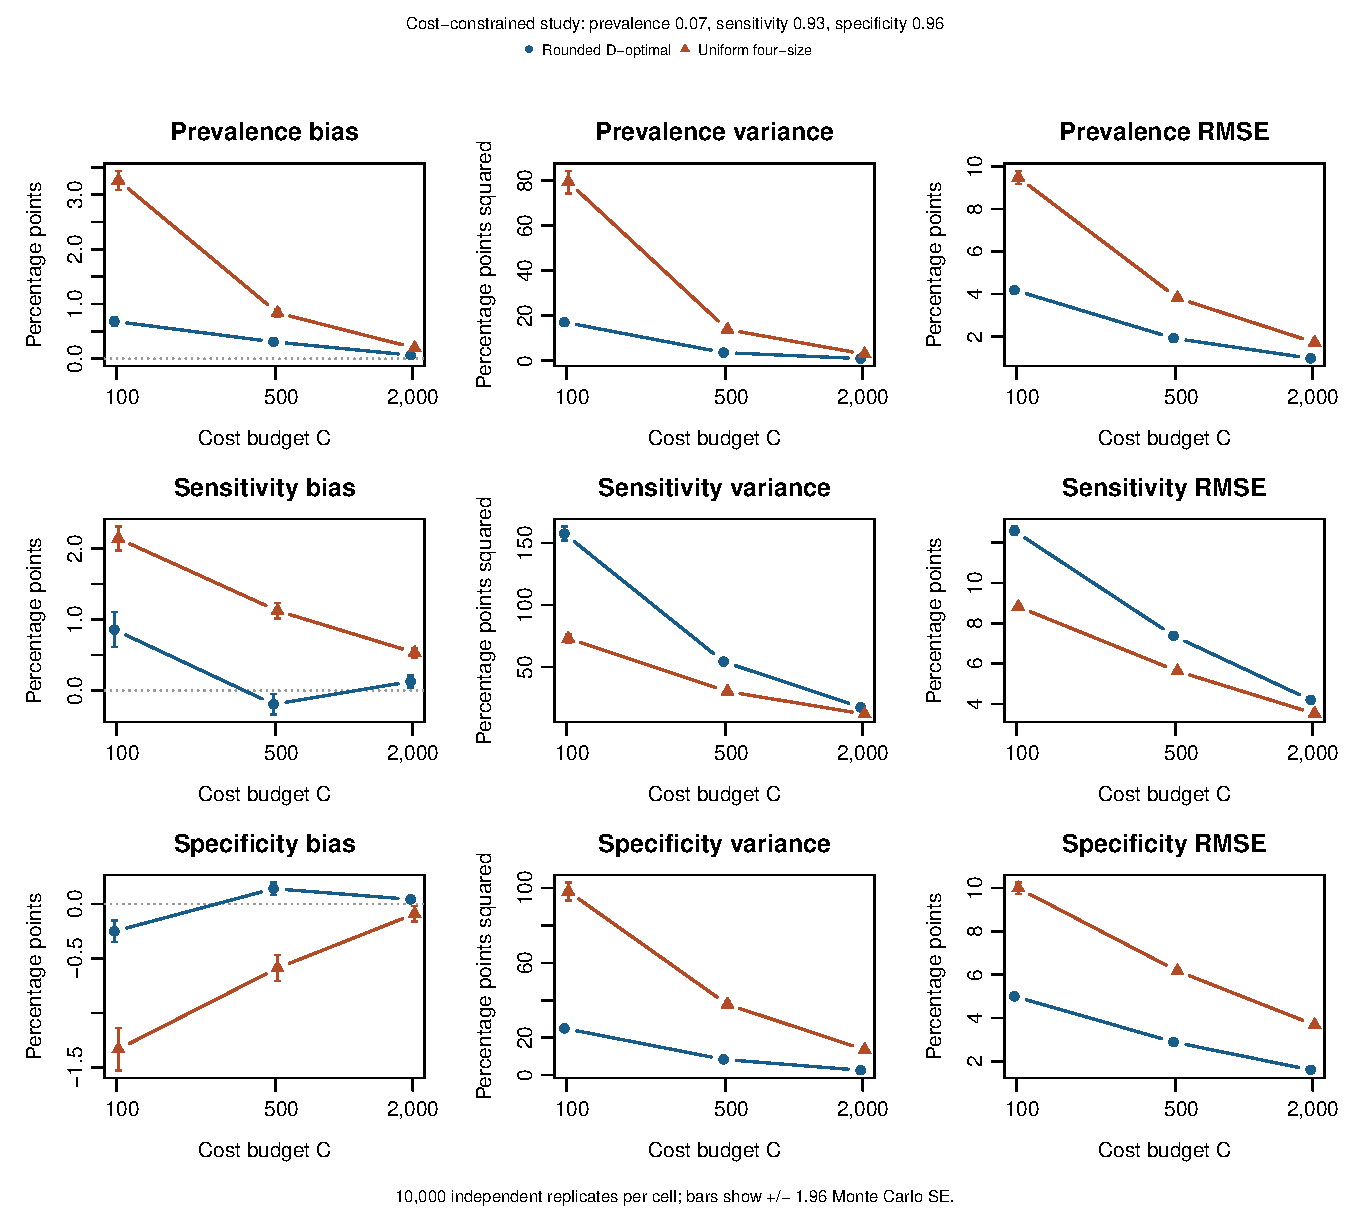
\includegraphics[width=.98\textwidth]{bias_cost.pdf}
\caption{Bias, variance and RMSE in the cost-budget setting. Bars show 1.96 Monte Carlo SEs on each side of the estimate. Small horizontal offsets separate the two designs.}\label{fig:bias-cost}
\end{figure}
\begin{figure}[!htbp]\centering
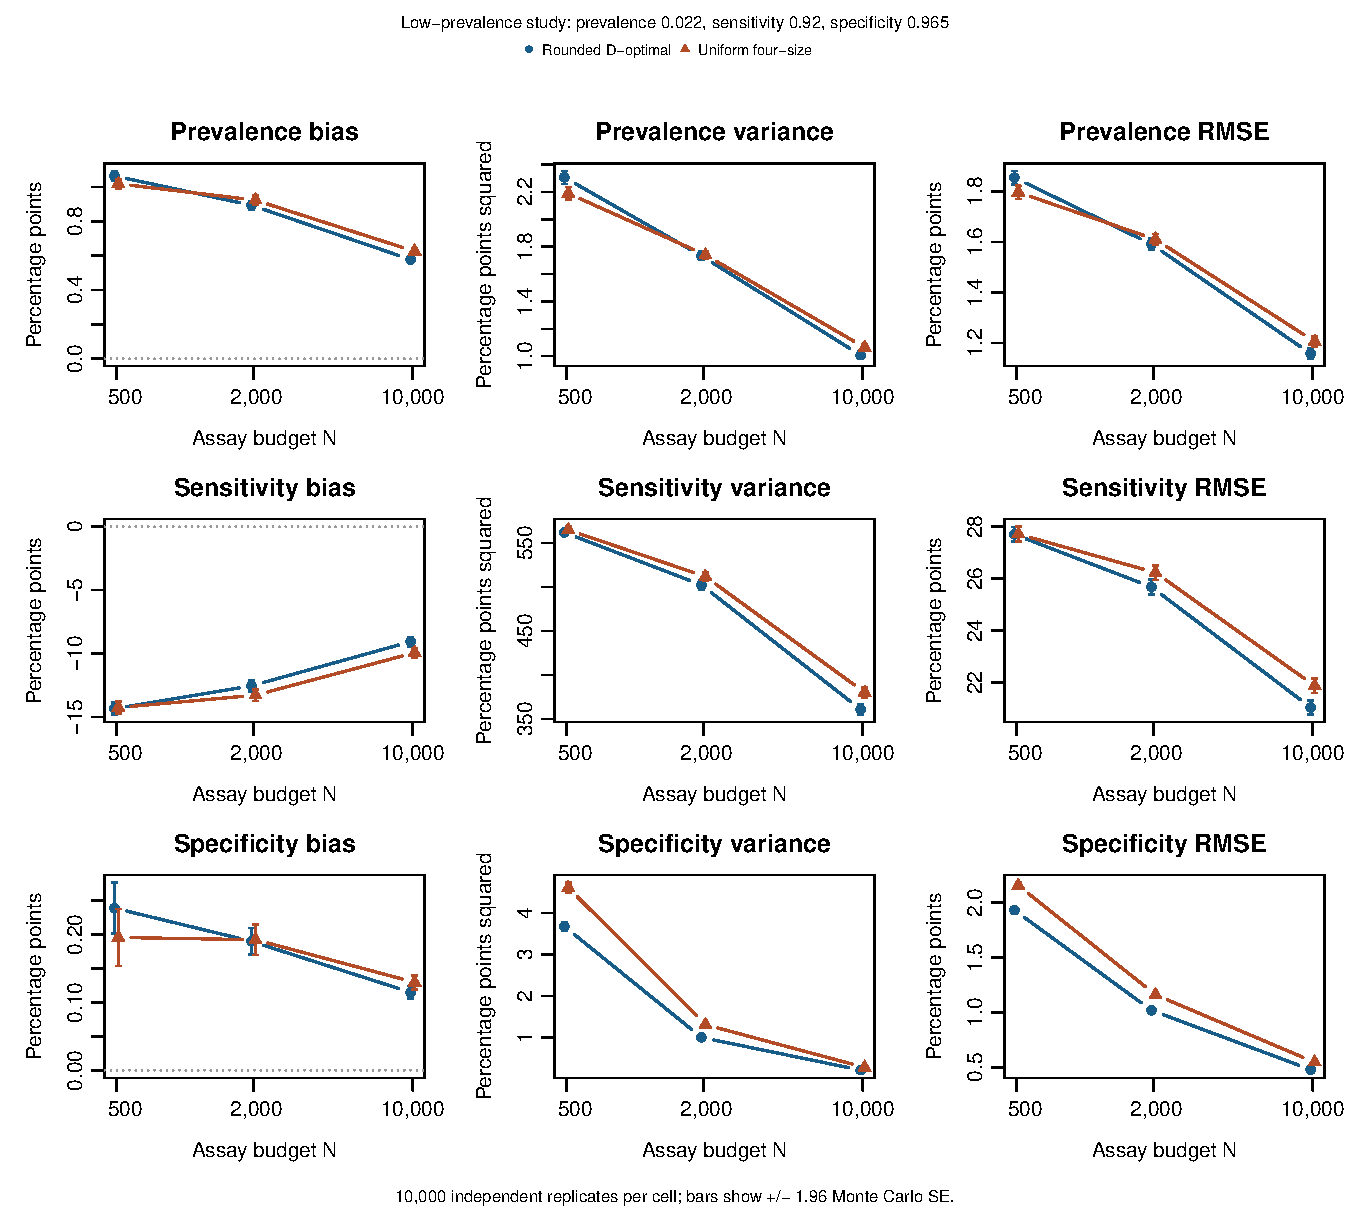
\includegraphics[width=.98\textwidth]{bias_low.pdf}
\caption{Bias, variance and RMSE in the low-prevalence setting. Bars show 1.96 Monte Carlo SEs on each side of the estimate. Small horizontal offsets separate the two designs.}\label{fig:bias-low}
\end{figure}

\FloatBarrier
\begin{thebibliography}{9}
\bibitem[Huang et~al.(2017)]{huang:2017:design-group}
S.-H. Huang, M.-N.~L. Huang, K.~Shedden and W.~K. Wong.
Optimal group testing designs for estimating prevalence with uncertain testing errors.
\emph{Journal of the Royal Statistical Society, Series B}, 79:1547--1563, 2017.
\bibitem[Hepworth and Biggerstaff(2021)]{hepworth:2021:bias}
G.~Hepworth and B.~J. Biggerstaff.
\newblock Bias correction in estimating proportions by imperfect pooled testing.
\newblock \emph{Journal of Agricultural, Biological and Environmental Statistics}, 26:90--104, 2021.
\newblock doi:10.1007/s13253-020-00411-5.

\end{thebibliography}
\end{document}
